\subsubsection{28.03.15 (Competition)}
\begin{center}
	2-nd day of competition "FTC Dutch Open"
\end{center}
Today there were qualification and final matches.\newline

Firstly, we talked with all teams again about the possibility of organising the alliance in final matches. After the shedule of qualification matches was announced, we discussed with teams, with whom we would play, our common strategy for a match.\newline

In parallel with communicating, we made program for the autonomus period from the parking zone. We couldn't make a program of autonomus from the ramp because of lack of time.\newline

All the teams in qualifications we divided into 2 divisions: Huygens and Laurence. In our division, Laurence, all teams had only three qualification matches because of troubles with wifi.\newline

Actions that we did in qualification matches:
\begin{enumerate}
	\item 1-st match:
	\begin{itemize}
		\item In autonomous period we put the balls into 30cm goal and 90cm goal (60 points).
		
		\item In tele op period all teams except our lost connection with the field. Unfortunately, we gave 90 cm rolling goal to our teammate, so we only filled with balls the 60 cm goal. (114 point).
		
		\item In the end game we moved 60 cm goal to the ramp, but our robot moved downwards from the ramp after the power was turned off. (30 points).
		
		\item Total: 204 points, we won. 
	\end{itemize}
	\item 2-nd match (In that match we had different software on our samantha, so we couldn't connect to the field. However, the judges didn't help us and we had to stay at the parking zone for the whole game):
	\begin{itemize}
		\item In autonomous period our teammate fell down from the ramp (20 points).
		
		\item In tele op period our team did nothing (0 points).
		
		\item In the end game our teammate moved the 30 cm goal to the parking zone. Also our robot stayed in the parking zone since the beginning of the match (20 points).
		
		\item Total: 40 points, it's hard to believe, but we won!
	\end{itemize}
	\item 3-rd match:
	\begin{itemize}
		\item In autonomous period (0 points).
		
		\item In tele op period (0 points).
		
		\item In the end game  (0 points).
		
		\item Total: 0 points
	\end{itemize}
	After the match, one of judges said us, that our mechaism for capturing rolling goals centers goals in a restricted way - it touchs the tube when riles allow only to touch the base. If we continue using this construction, we will get 1 minor for each game, so after we return from competition, we should remake the mechanism of centering goals.
\end{enumerate}


When were announced results of qualification matches it turned out that our team didn't reach the position in top-4 because of low score (although we won all matches). Likely, we were chosen to the final alliance by the "Auto Vortex" team. The final alliances consisted of 2 teams, so we played in all the matches.\newline

Strategy of our alliance:
\begin{enumerate}
	\item In the semi-final we fill 60 cm goal and lead goals to the ramp and "Auto Vortex" fills 90 cm goal and 120 cm goal.
	
	\item In the final game we decided to lose. The thing was that our opponents (the motherteam) were friends of the "Auto Vortex" team and they didn't have a quota for the world championship in St. Louis, when in our alliance we both already had. So, we decided to let them win, as it will be useful for us to have a one more friendly team on St. Louis Championship.
\end{enumerate}


Actions that we did in semi-final:
\begin{enumerate}
	\item 1-st round:
	\begin{itemize}
		\item In autonomous period (0 points).
		
		\item In tele op period (0 points).
		
		\item In the end game  (0 points).
		
		\item Total: 0 points
	\end{itemize}
	\item 2-nd round:
	\begin{itemize}
		\item In autonomous period (0 points).
		
		\item In tele op period (0 points).
		
		\item In the end game  (0 points).
		
		\item Total: 0 points
	\end{itemize}
\end{enumerate}

Actions that we did in final:
\begin{enumerate}
	\item 1-st round:
	\begin{itemize}
	    \item In autonomous period (0 points).
	
	    \item In tele op period (0 points).
	
	    \item In the end game  (0 points).
	
	    \item Total: 0 points
	\end{itemize}
	\item 2-nd round:
	\begin{itemize}
		\item In autonomous period (0 points).
		
		\item In tele op period (0 points).
		
		\item In the end game  (0 points).
		
		\item Total: 0 points
	\end{itemize}
	\item 3-rd round:
	\begin{itemize}
		\item In autonomous period (0 points).
		
		\item In tele op period (0 points).
		
		\item In the end game  (0 points).
		
		\item Total: 0 points
	\end{itemize}
\end{enumerate}


So our alliance won in category "Alliance-finalist".\newline

After the competition ended, we returned to the hotel and disassembled our robot for transportation.

Results of competition:
\begin{enumerate}
	\item We didn't take top places by the results of qualification matches.
	
	\item Our alliance won semi-final and lost final.
	
	\item We didn't gain prize in nomination "Engineering book".
	
	\item We didn't receive prize places in other nominations.
\end{enumerate}

Summing up:
\begin{enumerate}
	\item Success in competition:
	\begin{enumerate}
		
		\item We won 5 matches from 8 (3 qualification and 5 final matches).
		
		\item Our operators controlled the robot successfuly, worked competently and coordinated their actions with each other and with operators of ally, like at the previous competition in Moscow.
		
		\item Mechanisms worked steagily and didn't brake.
		
		\item Programme of autonomous period worked more stable, than at previous competition. However, we had problems with moving 30 cm goal to the parking zone because of weakness of additional capture for goal.
		
		\item Programme of tele op worked ok, but in 2 games game we had to use emergency power button to restart the servos, which didn't work.
		
	\end{enumerate}
	
	\item Our mistakes and disadvantages of construction:
	\begin{enumerate}
		\item Because of lags with translation of data, we wasted too much time trying to rise the bucket up to the needed height. We can solve this problem by automatization the moving of the lift. We can insert 4 positions: ground, 60 cm, 90 cm and 120 cm and use each of them by pressing one button.
		
		\item We also wasted some time on turning on the gripper for balls. During the game, we needed to stop it while the bucket is rised and then run it again. In our program the gripper automatically stops when the winch starts working, but to launch it we need to press the button on the joystick. That is the problem that when the wifi lags, we it's hard to check if it started working or not. So, to solve this problem, we need to automize working of gripper for balls and leave for operator only control of thew reverse for emergency situations.
		
		\item We scored 1 minor point in every final match because of forbidden construction of capture for rolling goals.
		
		\item After a few games we noticed, that one of the wheels is near to fall off besause the fixators were unable to withstand the load. So, we decided to install more fixators to the axles after the competition.
		
		\item Many robots on this competition were faster, than our and we know, that in USA robots are even faster than here, so we need to increase speed of our robot to be on equal footing with them. We can install gear for speed and try to take 2 motors from lift to wheel base because we use wheels constantly and the lift - only a few times per game.
		
	\end{enumerate}
	
	%\item Useful ideas that we took from other teams:
	%\begin{enumerate}
		%\item 
		%\begin{figure}[H]
		%	\begin{minipage}[h]{0.2\linewidth}
		%		\center  
		%	\end{minipage}
		%	\begin{minipage}[h]{0.6\linewidth}
		%		\center{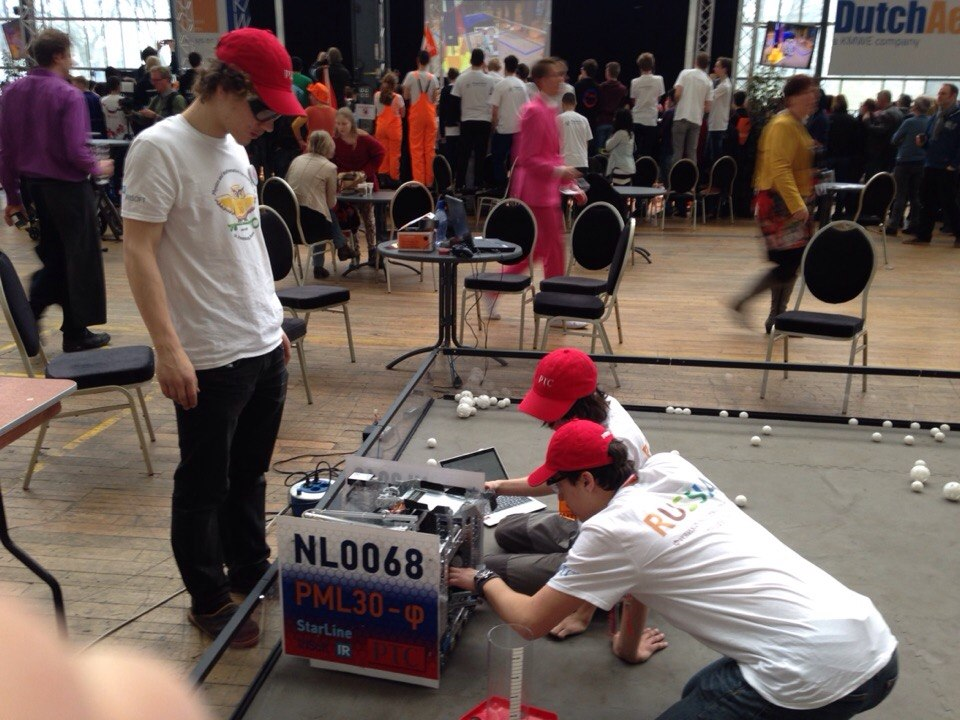
\includegraphics[scale=0.25]{days/28.03.15/images/02}}
		%		\caption{}
		%	\end{minipage}
		%\end{figure}
	%\end{enumerate}
	
	\item Tasks for the next meeting:
	\begin{enumerate}
		\item To make the mechanism that rise the rolling goal (the task that we hadn't realised from the previous competition).
		
		\item To make turning in autonomous period by giro (the task that we hadn't realised from the previous competition).
		
		\item Automise working of the lift and the gripper for balls.
		
		\item Remove slopes for centering goals from the mechanism for capturing rolling goals.
		
		\item Replace the self-made wire on the lift with a standard one.
		
		\item Make robot faster.
			
		\item Use 6 motors for motion and 2 for rising the lift.
		
		\item Remove the majority of friction between slats from the lift to make it move easier.
		
		\item Buy new strong servos and fix them on MOB (2 servos) and on the capture for goals (1 servo).
		
		\item To make the video for nomination "Compass Award".
		
		\item Fix the wheels more reliably.
		
	\end{enumerate}
	
\end{enumerate}
\fillpage